\documentclass[10pt,twoside,a4paper]{report}
\usepackage{amsmath}
\usepackage{amsfonts}
\usepackage{amssymb}
\usepackage{csquotes}
\usepackage{caption}
\usepackage{subcaption}
\usepackage[hidelinks]{hyperref}

% ETHASL package
% TODO Choose options according to your project
% som/bt/st/mt: Studies on Mechatronics, Bachelor Thesis, Semester Thesis, Master Thesis
% fs/hs: Spring term, Autumn term
% german/english: German/English
\usepackage[bt,fs,english]{packages/ethasl}

% Activate for german language
%\usepackage{german}
%\usepackage{ae}

%%%%%%%%%%%%%%%%%%%%%%%%%%%%%%%%%%%%%%%%%%%%%%%%%%%%%%%%%%%%%%%%%%%%%%%%%%%%%%%
% LaTeX preamble
%%%%%%%%%%%%%%%%%%%%%%%%%%%%%%%%%%%%%%%%%%%%%%%%%%%%%%%%%%%%%%%%%%%%%%%%%%%%%%%
% Encoding settings

% Paper size
\usepackage{a4}

% Headings
\usepackage{fancyhdr}

% More symbols
\usepackage{textcomp}\usepackage{gensymb}

% Math support for Times font
%\usepackage{txfonts}

% ISO date
\usepackage[english]{isodate}

% Multi column
\usepackage{multicol}

% Figures 
\usepackage{graphicx}

% Subfigures (obsolete)
%\usepackage{subfigure}

% Bibliography
\usepackage[numbers]{natbib}

% Clever references
\usepackage{cleveref}

% Nicer tables
\usepackage{booktabs}
\usepackage{array}
\usepackage{multirow}

% Colors
\usepackage{color}
\usepackage{colortbl}
\definecolor{black}{rgb}{0,0,0}
\definecolor{white}{rgb}{1,1,1}
\definecolor{darkred}{rgb}{0.5,0,0}
\definecolor{darkgreen}{rgb}{0,0.5,0}
\definecolor{darkblue}{rgb}{0,0,0.5}

% Additional math functionality
\usepackage{amsmath}
\usepackage{amssymb}

% Nice fractions
\usepackage{nicefrac}

% Upper case greek letters
\usepackage{upgreek}

% ISO math notation
\usepackage{isomath}
\renewcommand{\vec}{\vectorsym}
\newcommand{\mat}{\matrixsym}

% Units
\usepackage{units}

% Rotated objects
\usepackage{rotating}

% Indent
\setlength{\parindent}{0em}

% Include PDF pages
\usepackage{pdfpages}
\includepdfset{pages={-}, frame=true, pagecommand={\thispagestyle{fancy}}}

% Headings
\rhead[\thepage]{\nouppercase{\rightmark}}
\lhead[\nouppercase{\leftmark}]{\thepage}
\cfoot{}

% Links (last package)
\usepackage{url}
\usepackage{cleveref}


\title{Path Generation for a Mobile Drawing Robot}
%\subtitle{bla bla bla}

% TODO Add name of the authors
\studentA{Wolf Vollprecht}
% \studentC{Student 3}

% TODO Add name of the supervisors
\supervisionA{Nikolay Kobyshev}
\supervisionB{Philipp Krüsi}
%\supervisionC{Supervisor C}

% TODO Change if necessary
\projectYear{\the\year}
\begin{document}

%\maketitle
\pagestyle{plain}
\pagenumbering{roman}

\author{Wolf Vollprecht}
\title{Path Generation for a Mobile Drawing Robot}

%\chapter*{Preface}
\addcontentsline{toc}{chapter}{Preface}
%\chapter*{Vorwort}
%\addcontentsline{toc}{chapter}{Vorwort}

Bla bla \dots
%\cleardoublepage
%\chapter*{Abstract}
\addcontentsline{toc}{chapter}{Abstract}
%\chapter*{Zusammenfassung}
%\addcontentsline{toc}{chapter}{Zusammenfassung}

The BeachBot is a mobile, autonomous drawing robot for large scale sand art. Its primary purpose is the entertainment of beachgoers. The goal of this thesis was to develop and evaluate algorithms to automatically generate suitable trajectories to draw arbitrary images on the canvas. Main challenges have been to find a trajectory that reduces the drawing time and to make watching the drawing process appealing.

%\cleardoublepage
%\chapter*{Symbols}
\label{sec:symbols}
\addcontentsline{toc}{chapter}{Symbols}
%\chapter*{Symbolverzeichnis}
%\label{sec:symbole}
%\addcontentsline{toc}{chapter}{Symbolverzeichnis}

\section*{Symbols}
%\section*{Symbole}

\begin{tabbing}
 \hspace*{1.6cm} \= \kill
  $\phi, \theta, \psi$    \> roll, pitch and yaw angle \\[0.5ex] 					
  $b$                     \> gyroscope bias \\[0.5ex]										
  $\Omega_m$              \> 3-axis gyroscope measurement \\[0.5ex]   		
\end{tabbing}

\section*{Indices}
%\section*{Indizes}
\begin{tabbing}
 \hspace*{1.6cm}  \= \kill
 $x$ \> x axis \\[0.5ex]
 $y$ \> y axis \\[0.5ex]
\end{tabbing}

\section*{Acronyms and Abbreviations}
%\section*{Akronyme und Abkürzungen}
\begin{tabbing}
 \hspace*{1.6cm}  \= \kill
 ETH \> Eidgen\"ossische Technische Hochschule \\[0.5ex]
 EKF \> Extended Kalman Filter \\[0.5ex]
 IMU \> Inertial Measurement Unit \\[0.5ex]
 UAV \> Unmanned Aerial Vehicle \\[0.5ex]
 UKF \> Unscented Kalman Filter \\[0.5ex]
\end{tabbing}
%\cleardoublepage

%\tableofcontents

\pagestyle{fancy}
\pagenumbering{arabic}
\chapter{Introduction}
\section{The BeachBot Project}
The BeachBot project is a focus project at ETH Zurich. During two semesters of the bachelor studies, the team had the opportunity to develop a mobile and autonomous robot prototype for creating sand drawings on beaches (the final robot prototype is shown in \autoref{fig:beachbot}). In total 7 mechanical engineering students, one electrical engineering student and two industrial design students (from the Zürcher Hochschule der Künste) were working on the project. 

The result of the project is a three wheeled mobile robot that can drive autonomously. The key features are:
\begin{description}
\item[Localization] The robot is able to reliably localize itself on the beach, using a laser range finder and 3 or more reflective poles. The accuracy of the localization is about 3 centimetres.
\item[Driving speed and turning radius] The top speed of the robot is about 0.4 metres per second and it can turn on the spot. Both back wheels are independently steerable. The front wheel is also actuated. This is done to reduce the risk of getting stuck in sand.
\item[Rake] The main drawing tool of the robot is a rake. The rake consists of seven pin-pairs which are individually liftable.
\item[Controller] The controller uses the output from the localization to steer the robot so that it follows a pre-defined trajectory.
\item[Automatic Path Generation] An application was created to generate the trajectory for an arbitrary input drawing  that can then be drawn on the beach.
\end{description}

The robot has been successfully tested at the beach.

\begin{figure}
\centering
\begin{subfigure}[c]{1\textwidth}
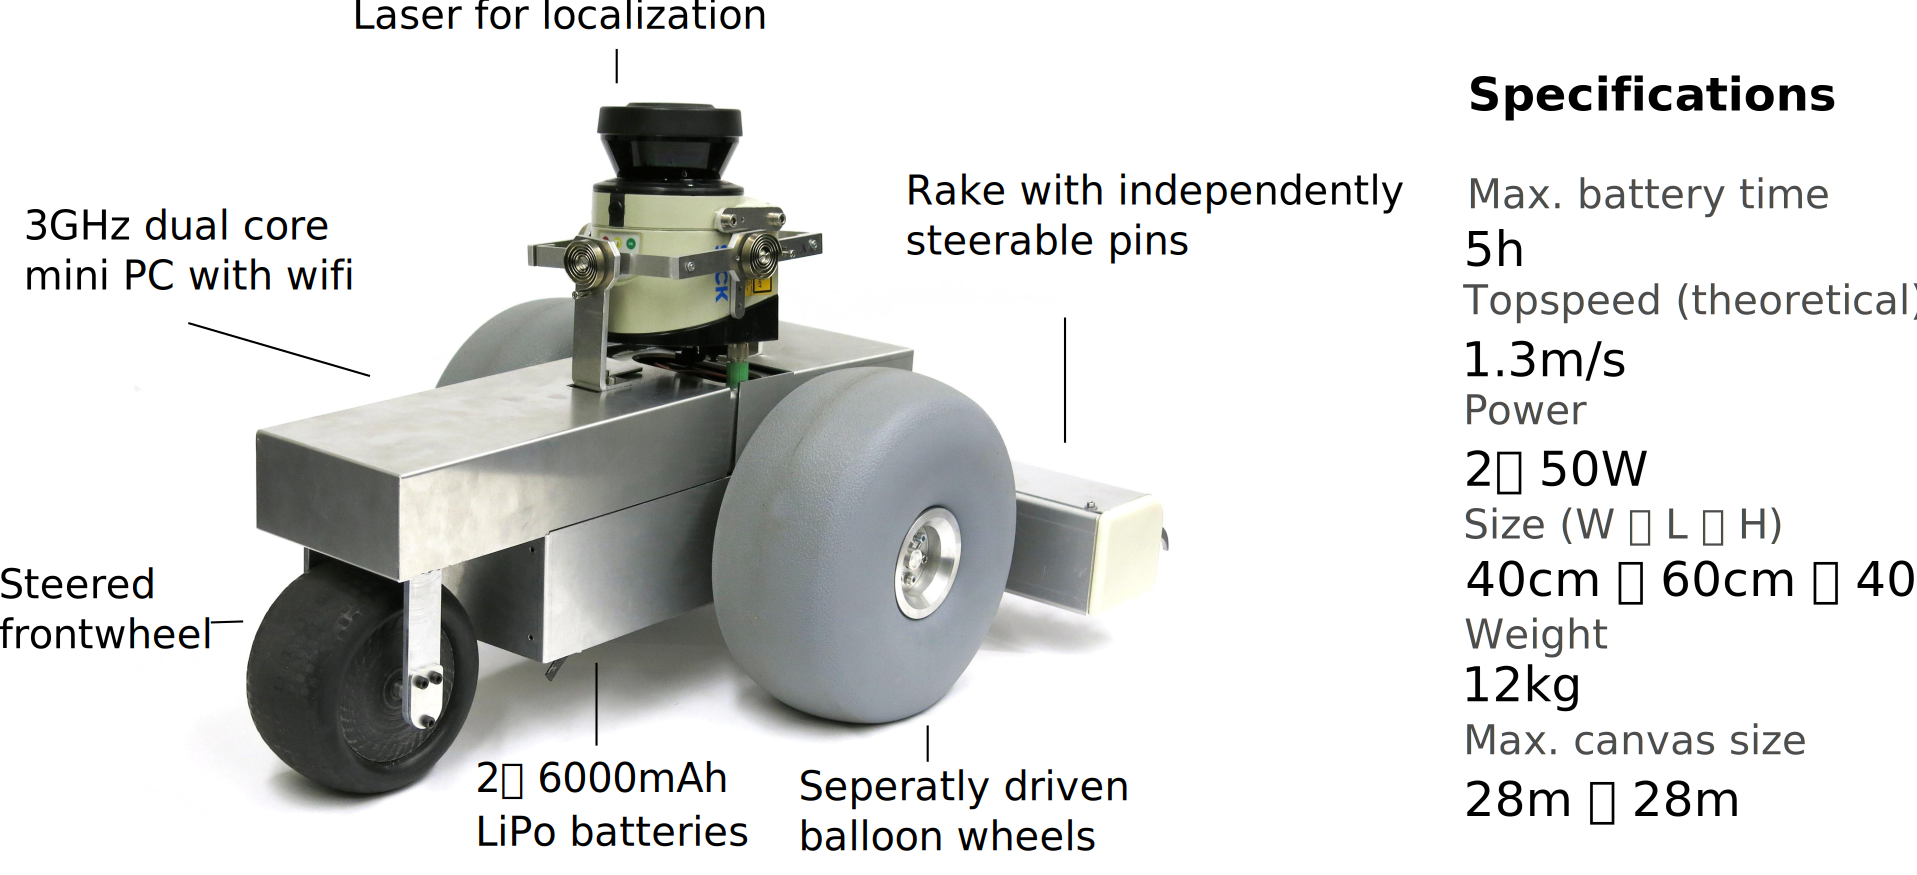
\includegraphics[width=\textwidth]{images/introduction/beachbot_spec.pdf} 
\end{subfigure}
\\
\begin{subfigure}[c]{1\textwidth}
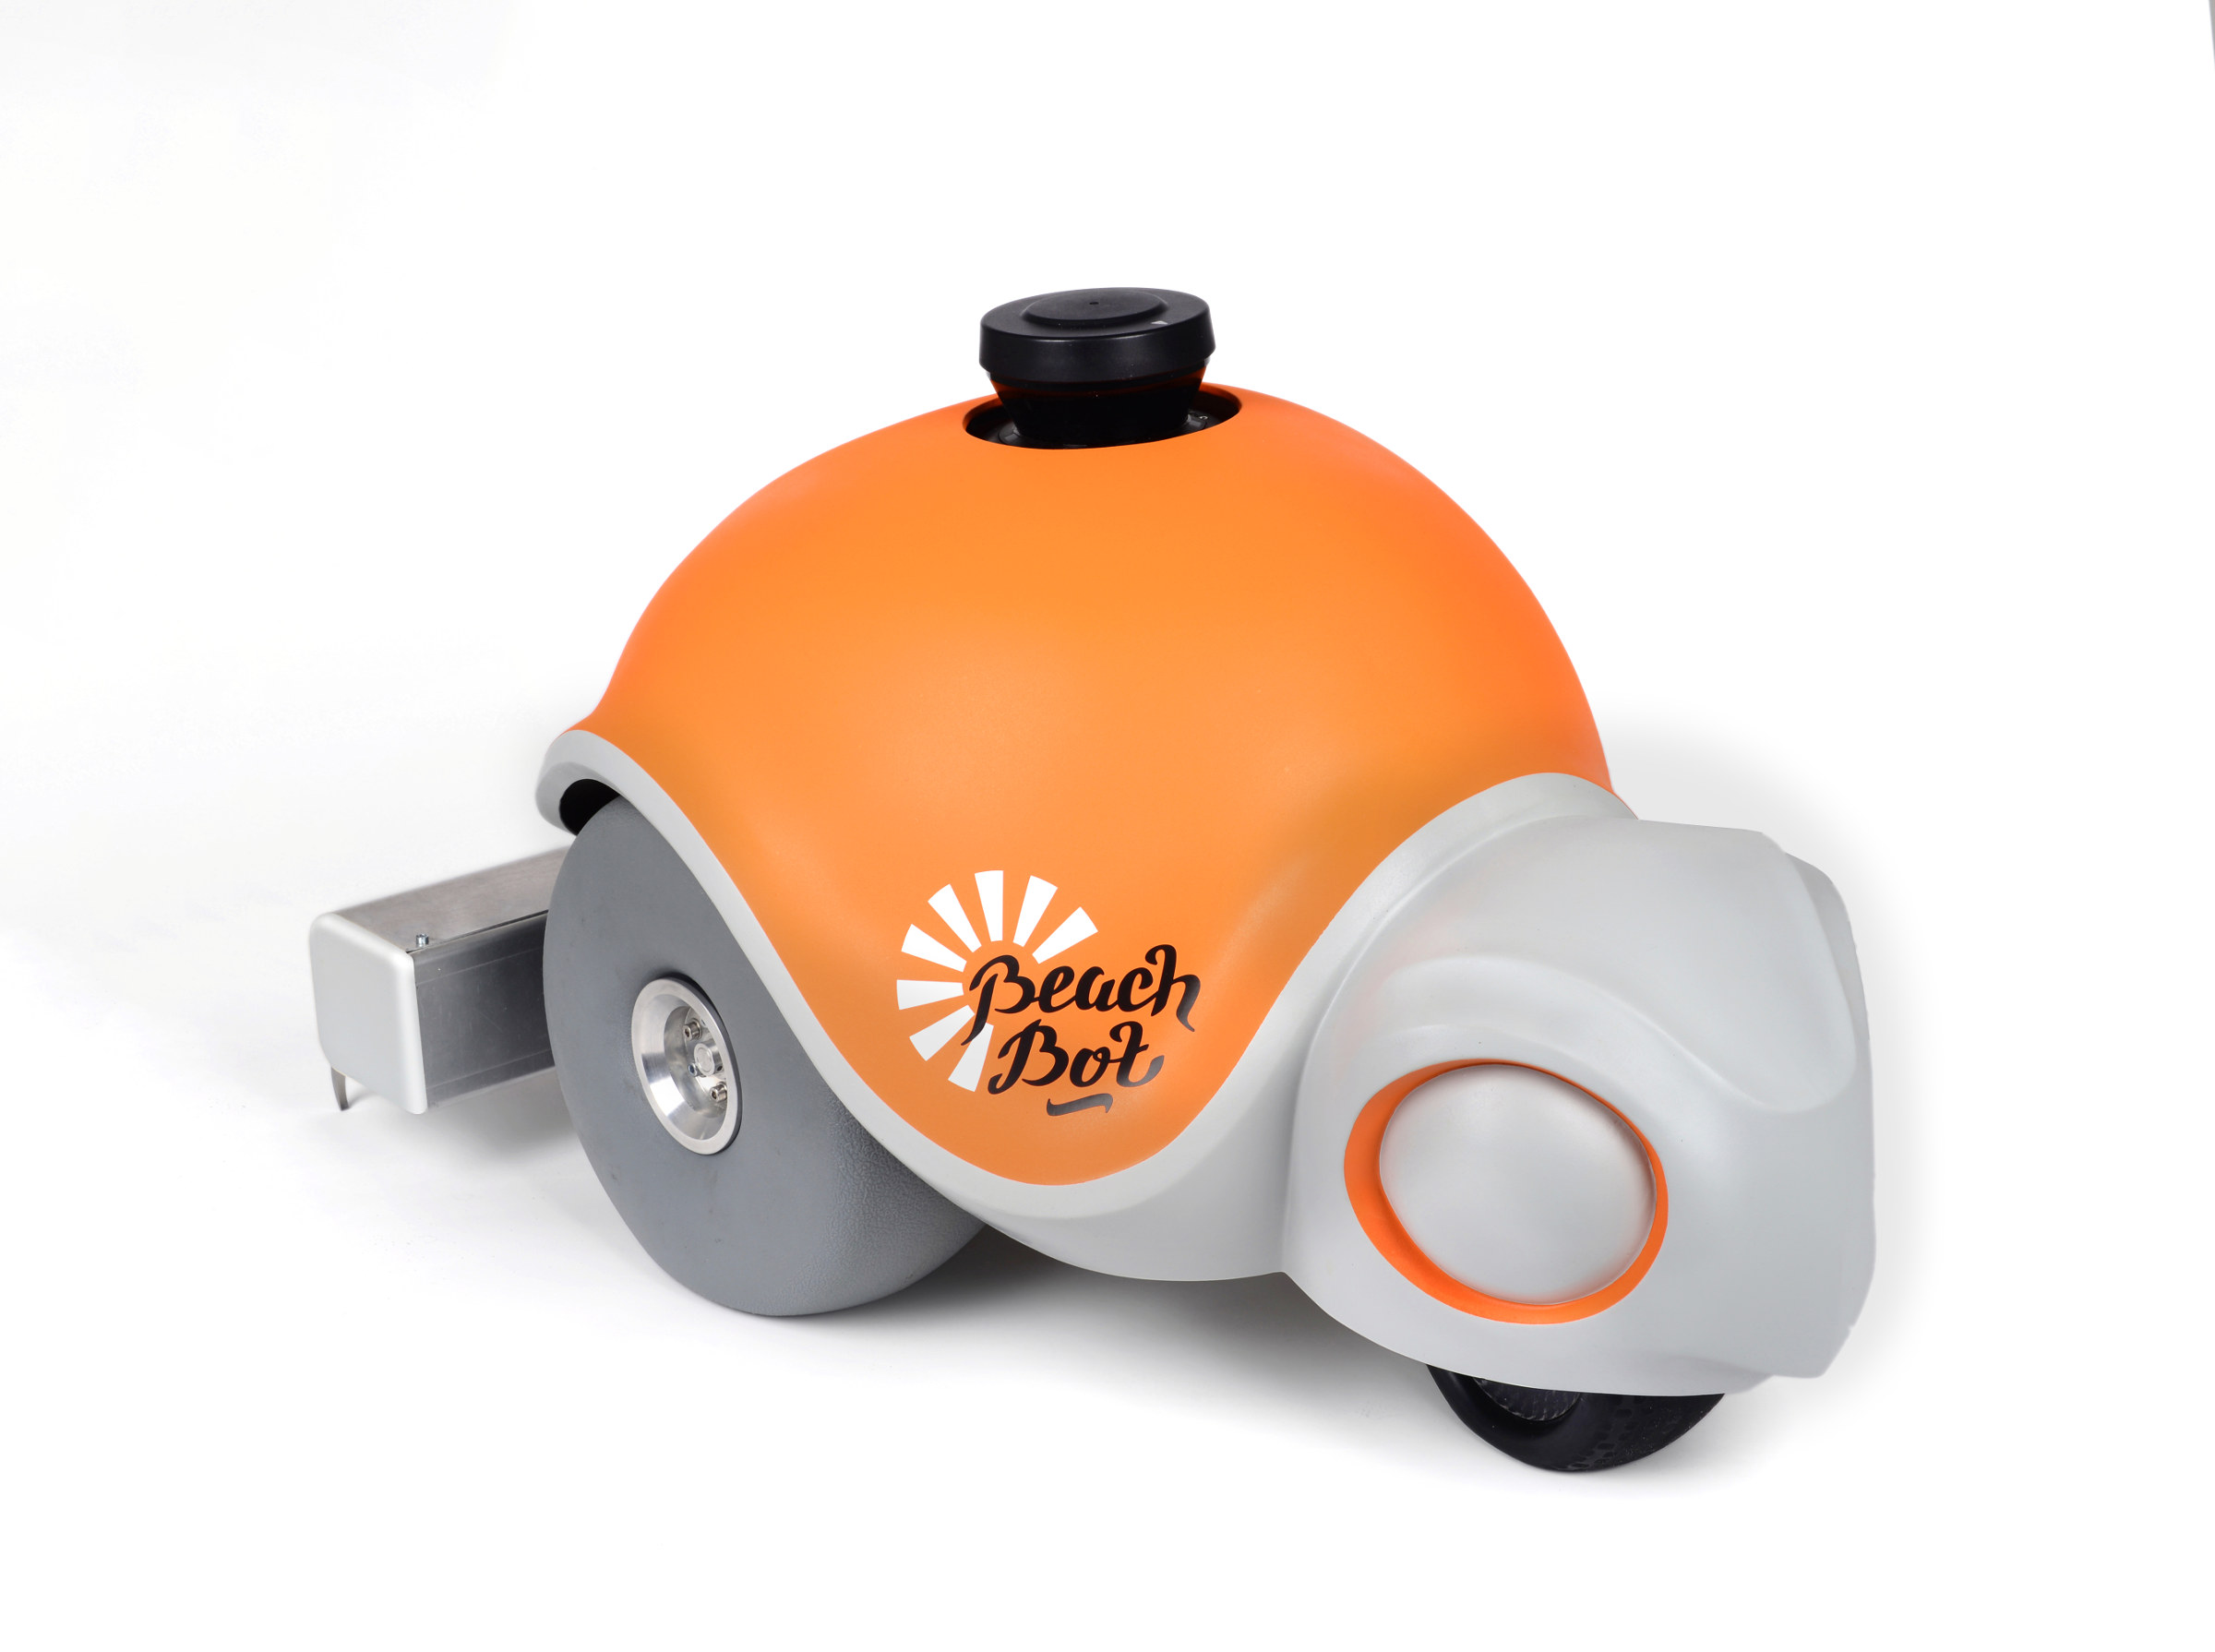
\includegraphics[width=\textwidth]{images/introduction/final_shell_scaled_down.jpg} 
\caption{The outer shell of the BeachBot}
\end{subfigure}
\\
\vspace{2cm}
\begin{subfigure}[c]{0.46\textwidth}
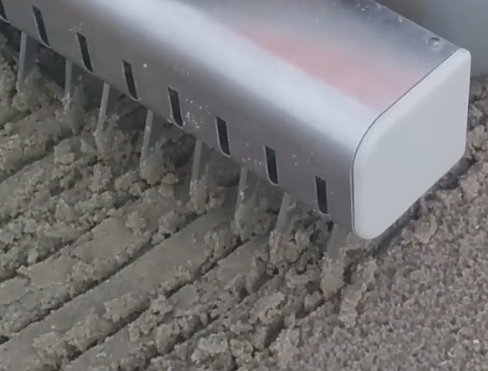
\includegraphics[width=\textwidth]{images/introduction/localization_precision.png} 
\caption{The rake in action}
\end{subfigure}
~~
\begin{subfigure}[c]{0.3\textwidth}
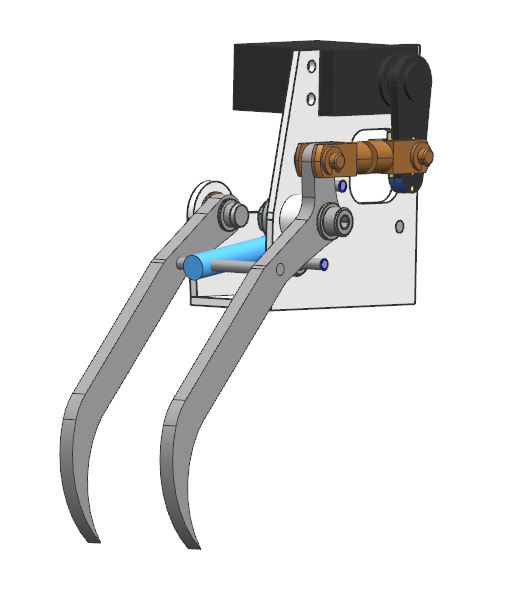
\includegraphics[width=\textwidth]{images/introduction/rake_pins.png}
\caption{One rake unit with servo motor and pin pair}
\end{subfigure}
\caption{Various images of the BeachBot}
\label{fig:beachbot}
\end{figure} 


\section{Requirements and Inspiration}

The BeachBot project itself was inspired by the images of sand artists like Peter Donnelly and Andres Amador, who create large scale sand art at beaches using a rake. Some of the imagery that we found online can be seen in \autoref{fig:sandart_inspiration}.

\begin{figure}
\centering
\begin{subfigure}[c]{1\textwidth}
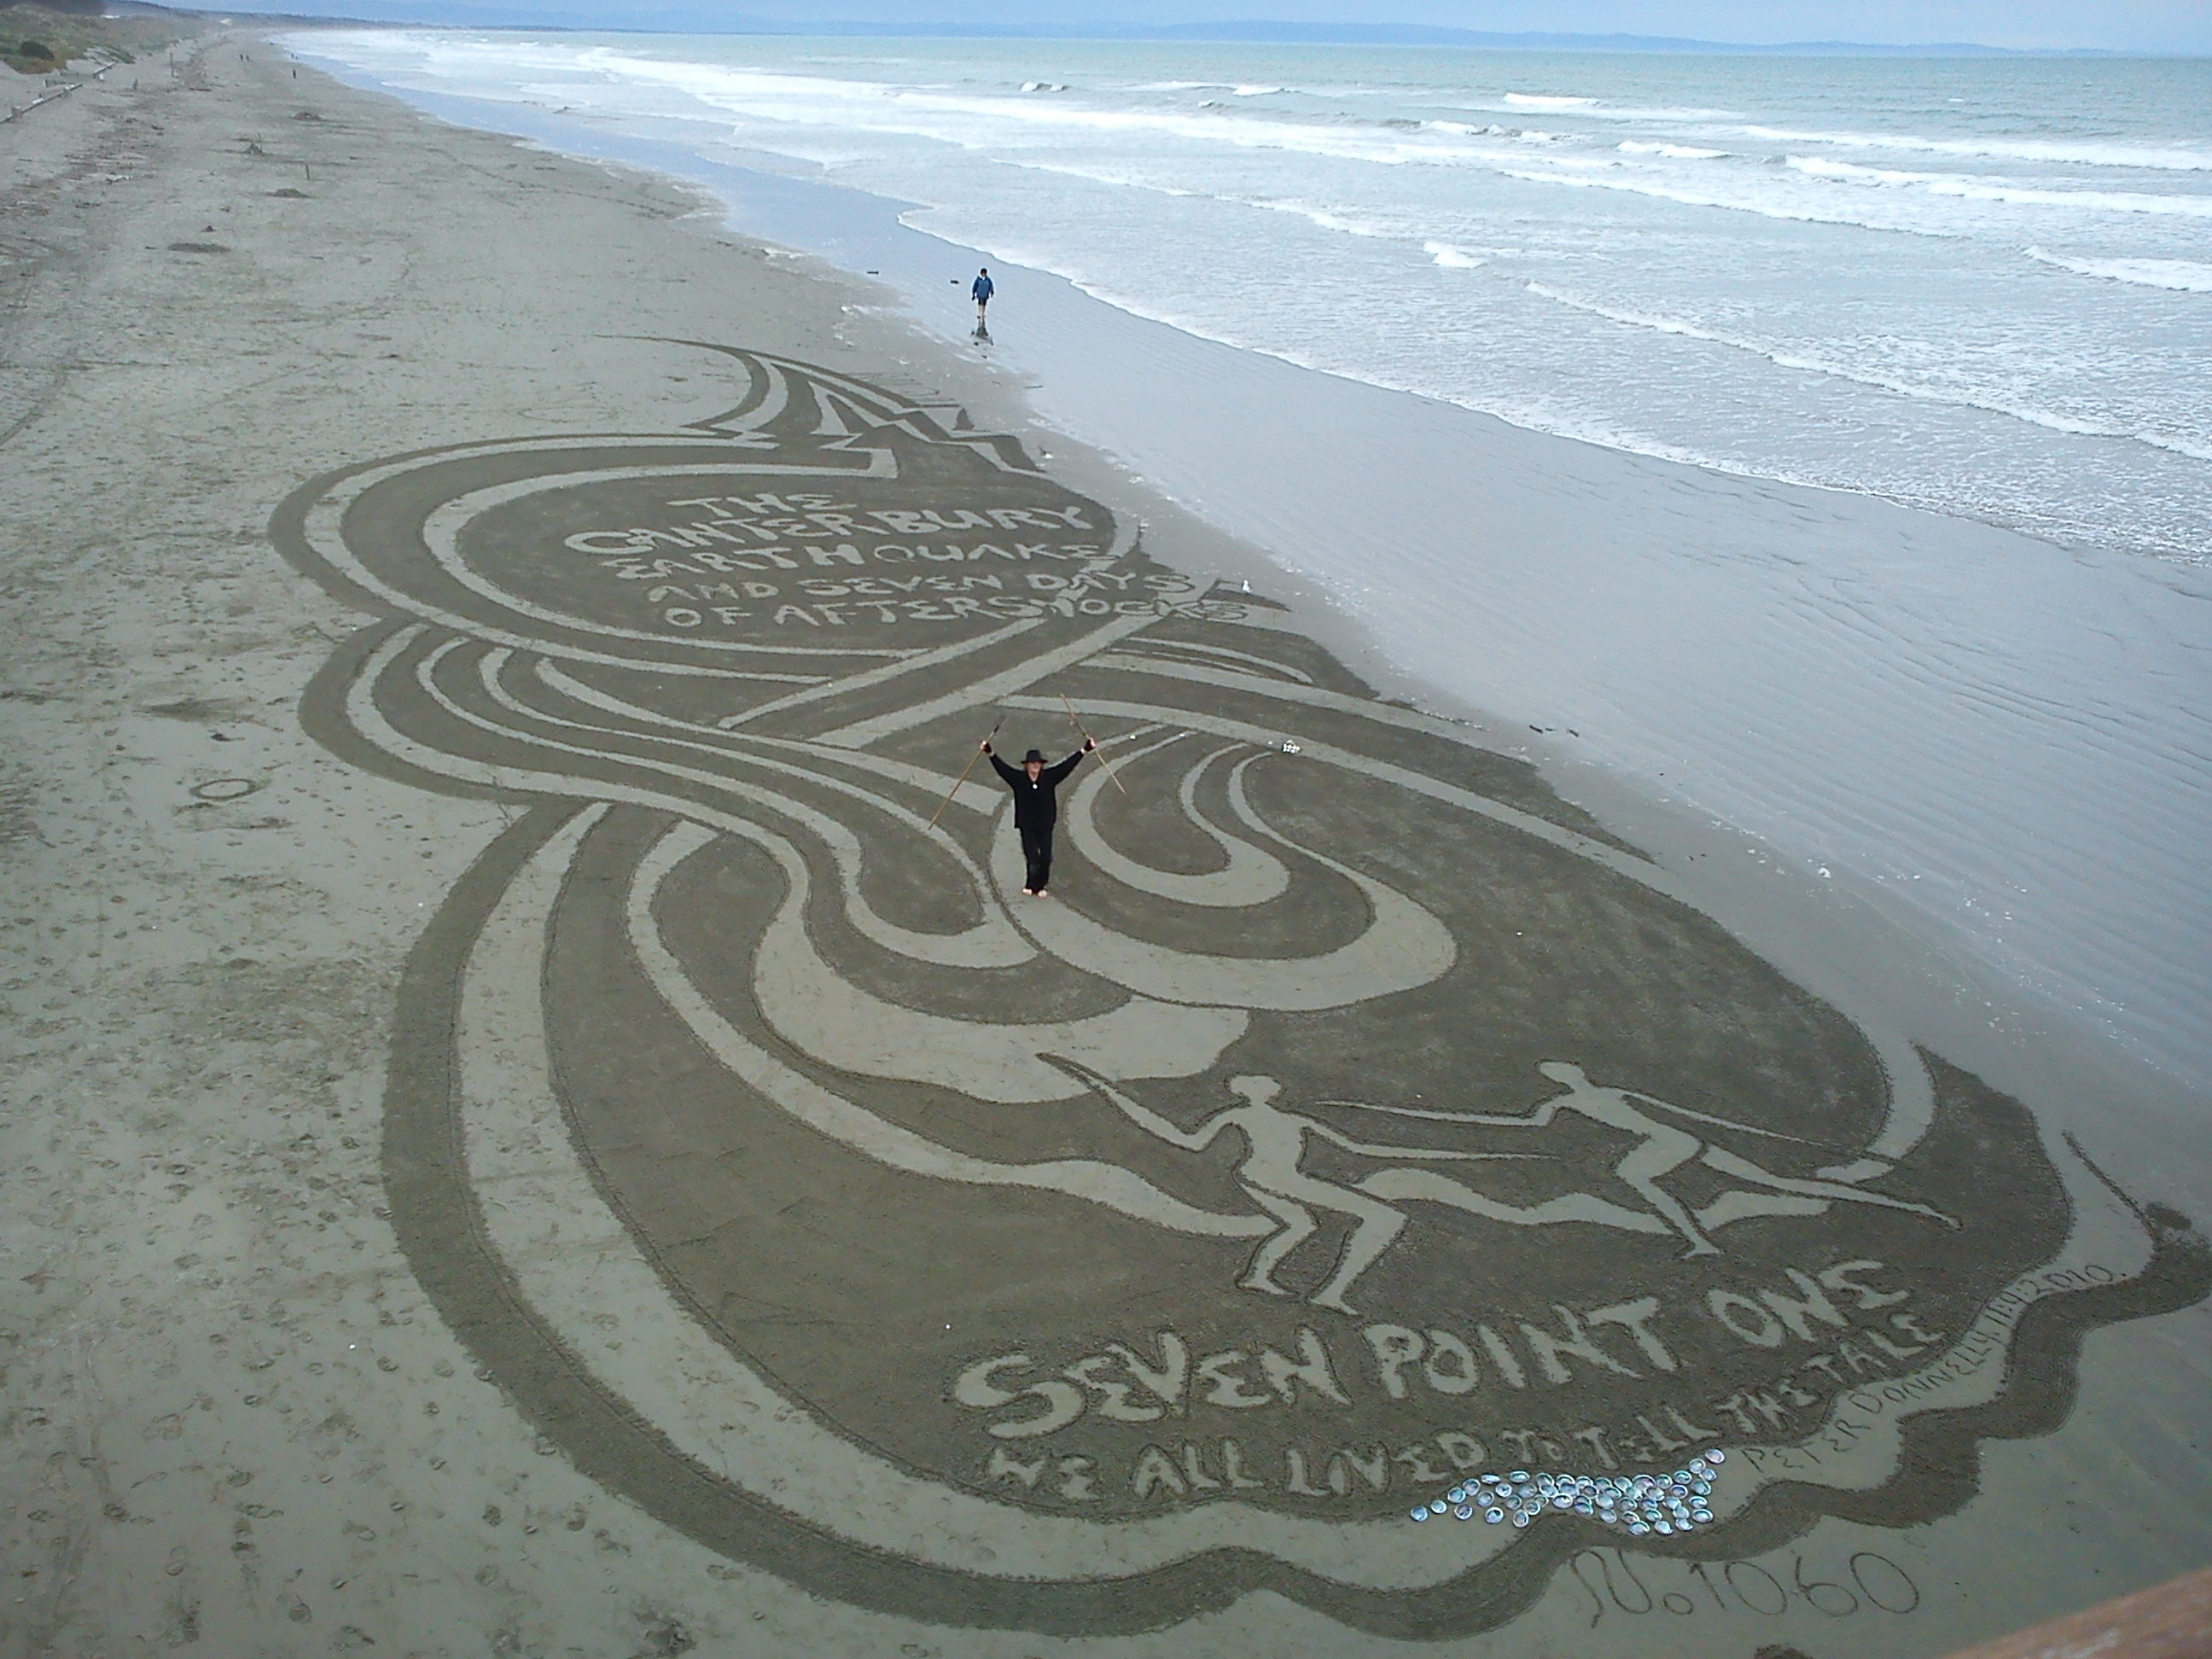
\includegraphics[width=\textwidth]{images/requirements_inspiration/donnelly_1.jpg} 
\caption{Sand drawing by Peter Donnelly. Source: \url{http://becky-garrett.blogspot.ch/2009/03/sand-dancer-peter-donnelly.html}}
\end{subfigure}
\\
\begin{subfigure}[b]{0.46\textwidth}
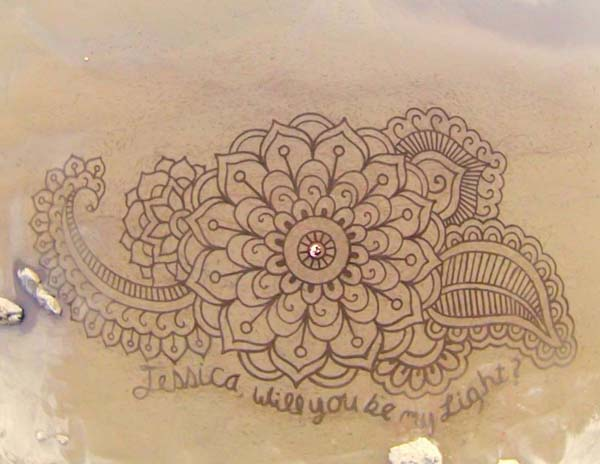
\includegraphics[width=\textwidth]{images/requirements_inspiration/andres_armador_1.jpg} 
\caption{Sand drawing by Andres Amador. Source: \url{http://sftimes.co/?id=25}}
\end{subfigure}
~
\begin{subfigure}[b]{0.46\textwidth}
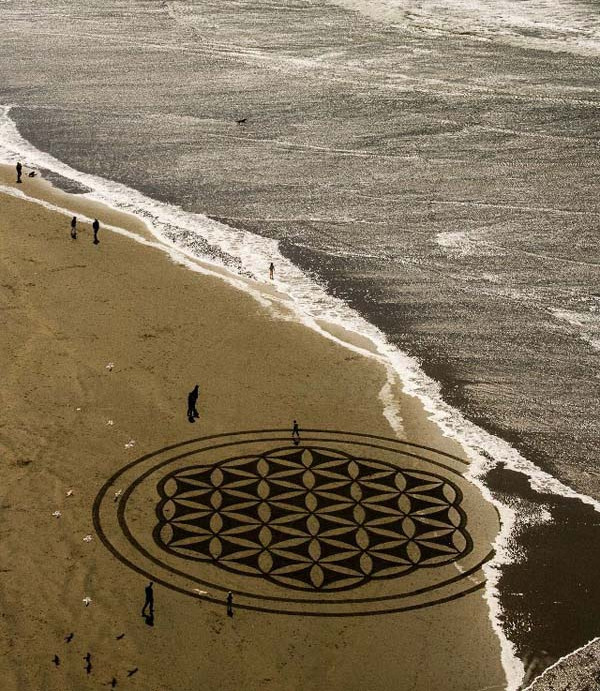
\includegraphics[width=\textwidth]{images/requirements_inspiration/andres_armador_2.jpg} 
\caption{Sand drawing by Andres Amador. Source: \url{http://sftimes.co/?id=25}}
\end{subfigure}
\caption{Various beach drawings by artists}
\label{fig:sandart_inspiration}
\end{figure}

Since our goal was to create drawings similar to those of the artists, we derived our requirements from these sample images.

First of all, the BeachBot should be able to draw lines. But more important is the support of filled areas. While it is relatively straightforward how lines or curves should be driven, there is no easy solution how to derive the path for filled areas. Not only should the area be covered to the highest extent, the drawing process should look interesting and artistic to spectators as well.

Derived from \autoref{fig:sandart_inspiration} is also the requirement that the BeachBot should only be able to draw in two colors. Gradients or differently colored areas are not needed.

Crossing lines or filled areas should be avoided as good as possible since the balloon wheels and the front wheel leave visible marks on the raked sand (a humanoid has a huge advantage here, since it can jump over the drawn areas). The effect of driving over the drawing depends on the scale. If the drawing is very big, it does not matter much if part of the image is crossed out. 

The input of the path generator should not only be computer readable, but also human editable. Typing in endless lists of coordinates would be tedious in the long run, and having a difficult format to work with would make it hard to collaborate with artists, for example. 
%Therefore the requirement to be able to use a modern graphics editor tool to work with was set. To conform to this requirement we soon decided to use \textit{Inkscape}\footnote{\url{http://inkscape.org}}, a popular open source vector graphics editor, as our input creation tool of choice. Further discussion about vector graphics as input and the steps to integrate a standardized vector graphics format into the path generator are explained in \autoref{sec:why_vector} and \autoref{sec:implementation_svg} respectively.

During the testing phase it was found out, that some of the generated paths needed some manual adjusting. To be able to easily edit the output of the generator program a graphical user interface should be created to work with the output of the generator program. 

In the following sections it will be shown how these requirements were fullfilled and to which extent.


% here you say that the project consists of a GUI and an algorithm.

\chapter{Path Planning Algorithms}
\section{Algorithm Overview}

The output of the path generator should be a single trajectory that completely connects and covers all elements of the drawing.

This happens in three steps: First, the polygons that have to be filled are selected and the fill algorithm is seperately executed for each of the polygons with polygon specific settings. In a second step all of the drawing elements are connected by an open tour and tries to minimize the traveled distance by applying a traveling salesman heuristic. As last step, connections with limited curvature are generated to complete the trajectory.

Each of those steps will be discussed in detail in this section.
% here you set the main requirements connected, as short as possible, no sharp angles etc)
\section{Image Structure}

Derived from the requirements, three different elements were identified as part of drawing (also shown in \autoref{fig:elements_def}:

\begin{description}
\item[Polyline] A line consisting of $2$ to $n$ vertices
\item[Polygon] A closed line, consisting of $2$ to $n$ vertices, where the last segment is a closing one. So that vertex $v_{n+1}$ equals $v_0$.
\item[Filled Polygon] Defined in the same way as the polygon, except that the inner space should be filled by the generated trajectory. Another difference is that the filled polygon can also contain holes, which should not be covered and be excluded from the fill trajectory.
\end{description}

\begin{figure}
\centering
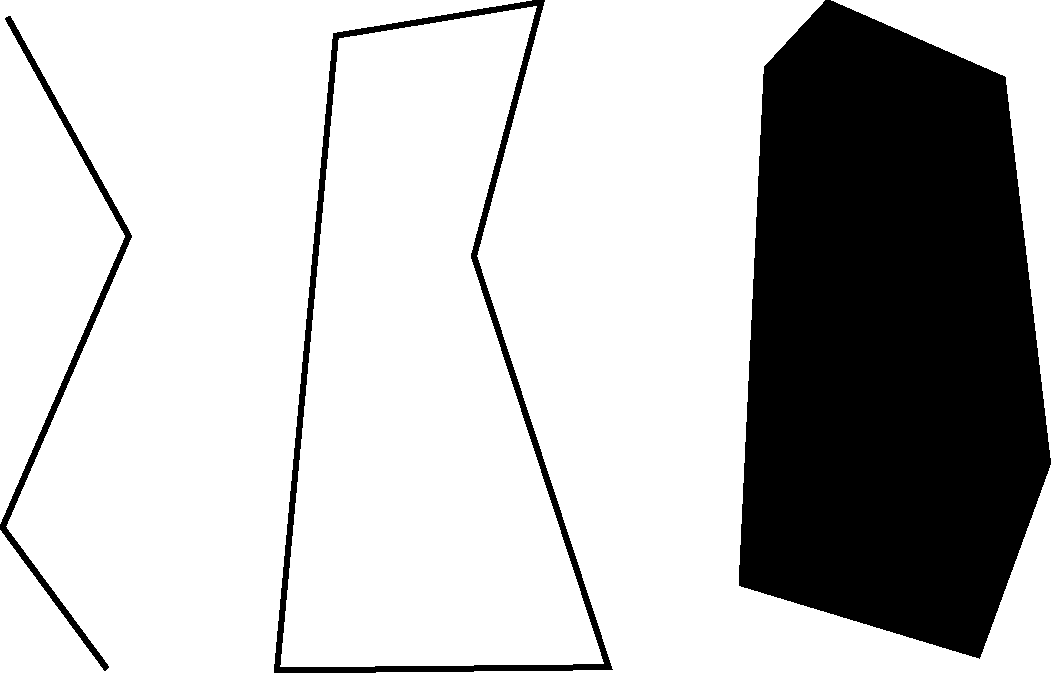
\includegraphics[width=0.6\textwidth]{images/path_planning/line_polygon_definition.pdf}
\caption{Polyline, polygon and filled polygon}
\label{fig:elements_def}
\end{figure}

% you discuss the lines, closed lines, filled polygons
% then you explain the structure that you work on elements separately and the connect them with TSP.
\section{Polygon Filling}

\subsection{Related Work}

Over time several surface coverage algorithms have been developed, and some distinctions can be made. 

Coverage algorithms exist for applications like autonomous vaccuum cleaners or autonomous lawn mowers, but also search and rescue robotic applications usually and they usually do not care if they visit the same spot twice. The target for those algorithms is rather to achieve complete coverage of an previously unknown terrain in sensible time. Usually, the complete surface coverage algorithms in are also connected with online map generation techniques \textit{SLAM}, whereas the path generation for the BeachBot should happen offline.

However, in agricultural applications some interesting algorithms have been found, which served as inspiration for the explorations presented in this thesis. Especially \citep{oksanen2007path}, who hinted at exploiting the straight skeleton algorithm to generate the inset polygons. An optimization strategy is employed to find the shortest trajectory through the field by repeatedly offsetting the remainding shape and traversing all possible ways off filling the shape. The algorithm is relatively computing intensive, what might be justified when using huge agricultural machines but what was not necessary for the goals of this thesis as the benefit of this optimization would be relatively small.

Another field where trajectories have to be generated is in \textit{Computer Aided Machining}. The process of removing layers of material from a block of metal is quite similar (though inverse, usually) to what is achieved in this thesis. Many publications deal with the problem of multi-axis milling machines which are far more complex and are also able to go over the machined surface without problem because they can lift the machnining head -- something that is not possible with the autonomous ground robot. 

One interesting publication in the CAM field is \cite{kao1998optimal} that presents a method to reduce gaps that are present when simply offsetting a polygon with spirals. The presented method could be a possible future improvement to the spiral fill algorithm of \autoref{sec:spiral_fill}.

The OpenCAM library has also been inspected...

	% all the algorithms go here
\subsection{Spiral Filling}

\subsubsection{Straight Skeleton}

To generate a spiral fill for the trajectory, we use the properties of the so called straight skeleton. The straight skeleton is defined as the topolgical skeleton of a polygon that is created by moving the edges inwards at a constant speed and observing the intersections of the vertices. It was first described by \citep{Aichholzer:jucs_1_12:a_novel_type_of}. 

During the creation of the straight skeleton, two events can happen: 

\begin{itemize}
\item Edge event: An edge shrinks to zero, making its neighboring edges adjacent now.
\item Split event: An edge is split, i.e., a reflex vertex runs into this edge, thus splitting the whole polygon. New adjacencies occur between the split edge and each of the two edges incident to the reflex vertex.
\end{itemize}
(cited from \citep{Aichholzer:jucs_1_12:a_novel_type_of}).

The straight skeleton is similar to the median axis of a polygon, but unlike the median axis it is not defined to have a constant distance to the polygon edges.

For the case of this thesis, the most interesting property of the straight skeleton is the ability to easily obtain inset polygons. The inset polygons are used to create a spiral fill for the polygons.




	% your algorithm
\subsection{Back and Forth Filling}
	% your algorithm. \subsubsection{Optimal Convex Partitioning} goes here without a special subsection for it

\section{Path Generation}
% state: we have 2 global problems
\subsection{Traveling Salesman Problem}
% general definition
% all three methods we tried, including LKH
\subsection{Adaptation of Traveling Salesman Problem for the Algorithm}
% how do you solve the problems of the closed loop in polygon and the constraint of returning to the start point

\section{Smooth line connections}
\subsubsection{Beziér Splines}
\subsubsection{Spiro Splines}

\chapter{Implementation}
\section{Input}	% svg files, why vector is better than raster
\section{SVG Parser}
\section{Tree Container}
\section{Preprocessing}
\section{Implementation of the Algorithms}
\section{Postprocessing}
\section{User Interface}

\chapter{Conclusion}
\cleardoublepage

\appendix
\chapter{Appendix}
\label{sec:appendix}
\section{Installation}

The installation procedure for the installation of the path generator program under Ubuntu 14.04 is described below:

\begin{enumerate}
\item For running the application, the following dependencies have to be satisfied:
\texttt{libcgal-dev, libboost1.54.0-all-dev, python2.7, libpython2.7-dev, build-essential, libeigen-dev, libjsoncpp-dev}. If the QT frontend should be installed, \texttt{libqt4-dev} has to be available. To be able to run the python server, the \texttt{flask} python library needs to be installed.
\item Cloning the source code from \url{https://github.com/asl-beachbot/pathmaker}: \texttt{git clone https://github.com/asl-beachbot/pathmaker}.
\item Running \texttt{cmake} with configuration options: \texttt{-DNOGUI=[ON/(OFF)]}, \texttt{-D32BIT=[ON/(OFF)]}. Round brackets indicate default value.
\item If \texttt{cmake} was run successfully, \texttt{make} can produce either the python module by using the target \texttt{python/beachbot\_pathgen} or the standalone target, called \texttt{svg\_parser} by calling e.g. \texttt{make svg\_parser -j3}.
\item If python version was built, starting the python server by calling \texttt{python python/server.py}.\\
If standalone version was built, \texttt{./svg\_parser} will launch the standalone program.
\item The HTML interface is accessed by opening the file \texttt{interface/index.html} in a recent version of the \textit{Firefox} or \textit{Chromium} web browser (server has to run).
\item To change the drawing that is opened by the server, change the file \texttt{assets/fill\_test.svg}. All sample files are also located at \texttt{assets/*.svg}.
\end{enumerate}
\newpage
\paragraph{Command Line Flags}
Command line flags can either be set as flags when the program is executed or can be set in the config file (the default file is \texttt{config.cfg} and \texttt{pythoncfg.cfg} for the server).
The list of allowed options is:
\small \\
\texttt{
  -h [ --help ]                        produce help message\\
  -f [ --filename ] arg                SVG File for parsing\\
  -r [ --round\_radius ] arg            set radius for corner rounding\\
  -m [ --fill\_method ] arg             set fill method (1: wiggle or 2: spiral)\\
  -s [ --scale\_for\_disp ] arg          scale for display\\
  --angle\_step arg                     Interpolation stepsize for rounding \\
                                       (e.g. 0.2 * PI)\\
  -m [ --max\_interpol\_distance ] arg   Max distance for points \\
  -d [ --display ]                     Open up the QT Window for inspection\\
  -t [ --threshold\_round\_angle ] arg   Defines from which angle on it should be rounded (or outer rounded)\\
  -l [ --line\_distance ] arg           Line distance inside filled elements\\
  --area\_deletion\_threshold arg        Maximum area of filling elements that will get deleted \\
  -c [ --config\_file ] arg             Use a different config file\\
  --segmentation\_on arg                Turn on or off segmentation\\
  --text\_export\_filename arg          Filename for export to textfile\\
  --svg\_export\_filename arg            Filename for export to SVG File\\
  --field\_width arg                    Width of field\\
  --field\_height arg                   Height of field\\
  --field\_offset arg                   Offset (margin) of field\\
  --segment\_offset arg                 Offset of Segment (from partitioning)\\
  --no\_tree\_ordering  Disables ordering of the tree (Useful when manual image from Timo!)\\
  --number\_segments\_bezier\_connect arg Define the number of segments for bezier interpolation)\\
  --stop\_go\_outer                      Round (and outer round) outer contours
                                       or stop-turn-go cycle?\\
  --round\_connection\_threshold         Threshold for rounding connections 
                                       (otherwise just place point) [squared 
                                       length of point distance]
}
\normalsize
\cleardoublepage

\bibliographystyle{ieeetr}
\bibliography{bibliography/references}
\addcontentsline{toc}{chapter}{Bibliography}

\end{document}
